\documentclass[conference]{IEEEtran}
\IEEEoverridecommandlockouts
% ---------------------------------------------------------------
% EE2000: Signal Processing, Fall 2026 -- Preliminary Project Report
% Indian Institute of Technology Hyderabad
%
% INSTRUCTIONS BEFORE SUBMITTING:
%  1. Replace <GROUP NUMBER> in the file name and \groupnum below.
%  2. Replace all author names / roll numbers in the \author block.
%  3. Compile the PDF and rename it exactly as: PPR-<group number>.pdf
% ---------------------------------------------------------------
\usepackage{cite}
\usepackage{amsmath,amssymb,amsfonts}
\usepackage{algorithmic}
\usepackage{graphicx}
\usepackage{textcomp}
\usepackage{xcolor}
\usepackage{tikz}
\usetikzlibrary{shapes.geometric,arrows.meta,positioning}
\usepackage{booktabs}
\usepackage{multirow}
\usepackage{url}
\usepackage[hidelinks]{hyperref}

\newcommand{\groupnum}{XX} % <-- replace XX with your group's serial number

\def\BibTeX{{\rm B\kern-.05em{\sc i\kern-.025em b}\kern-.08em
    T\kern-.1667em\lower.7ex\hbox{E}\kern-.125emX}}

\begin{document}

\title{Voice-Based Screening of Laryngeal Pathology Using Acoustic Signal Processing and Real-Time FPGA Implementation}

\author{
\IEEEauthorblockN{Student Name 1\IEEEauthorrefmark{1}, Student Name 2\IEEEauthorrefmark{1}, Student Name 3\IEEEauthorrefmark{1}, Student Name 4\IEEEauthorrefmark{1}}
\IEEEauthorblockA{\IEEEauthorrefmark{1}Department of Electrical Engineering, Indian Institute of Technology Hyderabad, India \\
Group \groupnum, EE2000: Signal Processing, Fall 2026 \\
Email: \{rollnumber1, rollnumber2, rollnumber3, rollnumber4\}@iith.ac.in}
}

\maketitle

\begin{abstract}
Laryngeal cancer is highly treatable when detected early, yet its principal warning sign, persistent hoarseness, is routinely dismissed until the disease has progressed, largely because definitive diagnosis requires an invasive laryngoscopic examination performed by a specialist. This project investigates whether short, non-invasive voice recordings can be used to flag laryngeal pathology through classical acoustic signal processing rather than end-to-end deep learning, so that the resulting system remains interpretable, lightweight, and deployable on resource-constrained hardware. We formulate the problem as a binary classification task that separates pathological (with a specific focus on malignant and pre-malignant) laryngeal conditions from healthy phonation, using sustained vowel recordings from the publicly available Saarbr\"ucken Voice Database (SVD) as our primary corpus. Our pipeline extracts classical time- and frequency-domain descriptors, jitter, shimmer, harmonics-to-noise ratio (HNR), mel-frequency cepstral coefficients (MFCCs), and cepstral peak prominence (CPP), and feeds them to a compact, interpretable classifier, mirroring the signal-processing-first philosophy of the course rather than treating the raw waveform as an opaque input to a large network. Each feature is a well-established, clinically documented acoustic biomarker, so that every stage of the pipeline remains explainable to a non-specialist audience rather than resting on a technique that only part of the team can defend. We further outline a plan to accelerate the feature-extraction stage on a Xilinx Spartan-7 FPGA, motivated by the goal of a real-time, low-power, point-of-care screening prototype. This report presents the problem statement, a review of eleven relevant works on voice-pathology and laryngeal-cancer detection, and the roadmap we will follow toward the mid-term and final submissions.
\end{abstract}

\begin{IEEEkeywords}
laryngeal cancer, voice pathology detection, acoustic signal processing, MFCC, jitter, shimmer, cepstral peak prominence, Saarbr\"ucken Voice Database, FPGA, biomedical signal processing
\end{IEEEkeywords}

\section{Introduction}

\subsection{Motivation}
Cancers of the larynx account for a substantial share of head-and-neck malignancies worldwide, and their five-year survival rate is strongly stage-dependent: tumours confined to the vocal folds and detected early are treated with radiotherapy or minimally invasive surgery at very high cure rates, whereas advanced-stage disease often requires total laryngectomy and carries a markedly worse prognosis. The earliest and most consistent symptom of laryngeal pathology, including malignant lesions, is a change in voice quality, most commonly persistent hoarseness (dysphonia). In practice, however, this symptom is nonspecific and is frequently attributed to benign causes such as laryngitis or vocal strain, so patients delay seeking care. The definitive diagnostic pathway, videostroboscopy or laryngoscopy followed by biopsy, requires a trained otolaryngologist, specialised equipment, and a clinic visit, resources that are unevenly distributed and largely inaccessible for routine population-level screening, particularly in rural and low-resource settings.

This gap motivates a screening layer that sits before the specialist visit: a tool that analyses a voice recording, obtainable from something as simple as a smartphone microphone, and flags a subset of patients whose voice characteristics are statistically consistent with pathological, and specifically malignant or pre-malignant, laryngeal conditions. Such a tool is not intended to replace laryngoscopic diagnosis; rather, it aims to triage referrals so that scarce specialist time is directed toward higher-risk patients sooner, while reassuring lower-risk patients without an invasive procedure.

\subsection{Problem Statement}
The goal of this project is to design and evaluate a signal-processing pipeline that classifies sustained-vowel voice recordings as \emph{healthy} or \emph{pathological}, with a specific emphasis on distinguishing \emph{malignant/pre-malignant} laryngeal pathology from \emph{benign} pathology and from healthy phonation, using features derived from classical acoustic signal processing rather than raw-waveform deep learning. Concretely, the project addresses three sub-problems:
\begin{enumerate}
    \item \textbf{Feature extraction}: computing a compact, clinically motivated set of acoustic biomarkers, jitter, shimmer, harmonics-to-noise ratio (HNR), fundamental frequency (F0) statistics, MFCCs, cepstral peak prominence (CPP), and spectral-envelope descriptors, from short sustained-vowel recordings. We deliberately restrict this stage to classical, well-documented features rather than more elaborate signal-decomposition techniques (e.g., glottal inverse filtering), so that the pipeline stays lightweight, fully interpretable, and realisable in real time on constrained hardware.
    \item \textbf{Classification}: training and evaluating classical machine learning classifiers (e.g., logistic regression, support vector machines) on these features to separate healthy, benign-pathological, and malignant/pre-malignant classes, and comparing this against deep-learning baselines reported in the literature.
    \item \textbf{Real-time realisation}: exploring hardware acceleration of the feature-extraction stage on a Xilinx Spartan-7 FPGA, to demonstrate that the pipeline can, in principle, run as a low-power, real-time embedded screening device rather than remaining a purely offline software model.
\end{enumerate}

This framing keeps the project rooted in signal processing, jitter/shimmer estimation, pitch tracking, filterbank-based cepstral analysis, and spectral estimation are all core DSP operations, while still connecting to a socially meaningful biomedical application, consistent with the ``Audio and speech processing'' and ``Biomedical applications'' themes listed in the course project flier.

\subsection{Report Organisation}
Section~\ref{sec:litreview} reviews eleven works spanning classical-feature-based and deep-learning-based voice pathology detection, the datasets they use, and the specific sub-problem of malignant-versus-benign discrimination. Section~\ref{sec:nextsteps} lays out our plan for the mid-term and final phases of the project, including the FPGA acceleration goal, and Section~\ref{sec:conclusion} concludes this preliminary report.

\section{Literature Review}
\label{sec:litreview}

\subsection{The Saarbr\"ucken Voice Database}
Nearly all the works reviewed below use the Saarbr\"ucken Voice Database (SVD), an open-source corpus assembled by the Institute of Phonetics at Saarland University, containing recordings from over 2000 speakers covering more than 70 documented voice pathologies \cite{harar2017}. Each recording session includes sustained phonation of the vowels /a/, /i/, and /u/ at normal, high, low, and rising-falling pitch, together with a short spoken sentence, sampled at 50\,kHz with 16-bit resolution; a parallel electroglottographic (EGG) signal is also available for a subset of recordings. A clinician-assigned pathology label accompanies every recording, which allows the eight malignant and pre-malignant conditions in the database (38 patients in total) to be separated from a much larger benign-pathology group and from healthy controls \cite{paterson2024}. This labelling structure is central to our project, since most prior work collapses ``pathological'' into a single class, whereas our problem statement specifically requires isolating the malignant/pre-malignant subset.

\subsection{Deep-Learning Approaches to Voice Pathology Detection}
Harar \emph{et al.} \cite{harar2017} were among the first to apply deep neural networks directly to raw SVD audio, combining convolutional layers with recurrent long short-term memory (LSTM) layers on 64\,ms Hamming-windowed segments of the sustained /a/ vowel. Their model achieved 68.08\% test accuracy with 66.75\% sensitivity and 77.89\% specificity, results the authors describe as promising but short of the state of the art, illustrating that raw-waveform deep learning on SVD is non-trivial without careful architecture design or a larger training set.

Mohammed \emph{et al.} \cite{mohammed2020} instead used a pre-trained convolutional neural network with transfer learning and a tailored training strategy on SVD, reporting substantially higher performance: 95.41\% accuracy, 94.22\% F1-score, and 96.13\% recall, with inference completed within three seconds, positioning their system as viable for real-time clinical use. Ksibi \emph{et al.} \cite{ksibi2023} proposed a two-level cascaded CNN--RNN architecture that first classifies speaker gender and then, conditioned on that outcome, classifies pathological versus healthy voice; this two-stage design improved on several earlier SVD results, reaching 88.84\% accuracy and an 87.39\% F1-score, and highlights that demographic conditioning (age, sex) is a useful auxiliary signal, consistent with SVD's inclusion of speaker metadata.

\subsection{Classical Feature-Based Approaches}
In contrast to end-to-end deep learning, Lee \cite{lee2021} evaluated feedforward and convolutional networks driven not by raw audio but by hand-crafted classical features, mel-frequency cepstral coefficients (MFCCs), linear prediction cepstral coefficients (LPCCs), and higher-order statistics (skewness and kurtosis of the signal distribution), extracted from 518 SVD recordings of the /a/, /i/, and /u/ vowels. The best configuration (a CNN classifier on LPCC features for the /u/ vowel in male speakers) reached 82.69\% accuracy, and the study found statistically significant differences in normalized skewness and kurtosis between healthy and pathological voices, supporting the use of such classical descriptors as discriminative features rather than merely pre-processing artefacts. This result is directly relevant to our approach, since it demonstrates that classical, interpretable acoustic features carry substantial diagnostic information even without an end-to-end deep network, and that feature choice interacts strongly with which vowel and speaker sex is analysed.

\subsection{Malignant-Specific Detection: The Closest Prior Work}
The work most directly aligned with our problem statement is the benchmark study by Paterson \emph{et al.} \cite{paterson2024}, which explicitly targets the benign-versus-malignant distinction rather than the more common healthy-versus-pathological split. The authors built a reproducible suite of 36 classifiers trained on the Far Eastern Memorial Hospital (FEMH) voice dataset and externally validated on SVD, comparing three feature representations, OpenSMILE acoustic features, MFCCs, and Wav2Vec2 deep embeddings, across support vector machines, multilayer perceptrons, and logistic regression, with and without demographic and symptom metadata. Their best model, logistic regression on OpenSMILE features combined with demographic and symptom information, achieved 83.7\% balanced accuracy and an AUROC of 0.918 on the FEMH holdout set. This paper is important to our project for two reasons: first, it confirms that malignant-versus-benign discrimination from voice alone is meaningfully harder than generic pathology detection (accuracy in the 80s rather than the 90s reported for coarser tasks); second, it shows that a classical-feature-plus-linear-classifier pipeline can be competitive with, and more interpretable than, deep embeddings for this specific task, which directly supports our decision to build the project around classical DSP features.

\subsection{Feature Engineering, Reproducibility, and Class Imbalance}
Several works address the practical challenges of working with SVD-style data. Islam \emph{et al.}~\cite{islam2022} combined convolutional neural networks with both electroglottographic and speech signals to improve robustness. A more recent reproducibility-focused study introduces a ``pitch-difference'' feature and a documented, openly released pipeline achieving 84.1\% unweighted average recall (UAR) under stratified cross-validation, explicitly addressing the small effective sample size of the malignant class by favouring simple, well-validated features over complex models. This concern is especially relevant to our project, since, as noted above, only 38 of the roughly 2000 SVD patients carry a malignant or pre-malignant label; any classifier we build must therefore explicitly address severe class imbalance, through resampling (e.g., SMOTE), class-weighting, or stratified evaluation, rather than reporting a raw accuracy figure that a trivial majority-class classifier could inflate.

\subsection{Summary and Identified Gap}
Table~\ref{tab:litsummary} summarises the reviewed works. Two gaps emerge that this project aims to address. First, the large majority of SVD-based studies treat the task as \emph{healthy vs.\ any pathology}, a coarser and easier problem than the \emph{benign vs.\ malignant} distinction that is clinically most valuable for cancer screening; only \cite{paterson2024} targets the malignant-specific problem directly, and it does so with classical features rather than a full DSP-motivated pipeline. Second, none of the reviewed works consider real-time or embedded deployment, every system reviewed is an offline software pipeline running on general-purpose hardware. Our project addresses the first gap by explicitly isolating the malignant/pre-malignant SVD subset as a target class, and the second by planning a Xilinx Spartan-7 FPGA implementation of the feature-extraction stage, as detailed in Section~\ref{sec:nextsteps}.

\begin{table*}[t]
\centering
\caption{Summary of reviewed literature on voice pathology and laryngeal cancer detection}
\label{tab:litsummary}
\begin{tabular}{@{}p{2.6cm}p{2.6cm}p{3.4cm}p{4.4cm}p{2.6cm}@{}}
\toprule
\textbf{Work} & \textbf{Dataset} & \textbf{Features} & \textbf{Method} & \textbf{Key Result} \\
\midrule
Harar et al. \cite{harar2017} & SVD (/a/ vowel) & Raw waveform & CNN + LSTM & 68.08\% test accuracy \\
Mohammed et al. \cite{mohammed2020} & SVD & Deep (pretrained CNN) & Transfer-learning CNN & 95.41\% accuracy \\
Ksibi et al. \cite{ksibi2023} & SVD & Hand-crafted + deep & Two-level CNN--RNN (gender-conditioned) & 88.84\% accuracy \\
Lee \cite{lee2021} & SVD (518 samples) & MFCC, LPCC, HOS & FNN / CNN & 82.69\% accuracy (best config.) \\
Paterson et al. \cite{paterson2024} & FEMH (train), SVD (external test) & OpenSMILE, MFCC, Wav2Vec2 & Logistic regression, SVM, MLP & 83.7\% balanced accuracy, AUROC 0.918 \\
Islam et al. \cite{islam2022} & SVD + EGG & Speech + EGG signals & CNN & Improved robustness via multimodal fusion \\
\bottomrule
\end{tabular}
\end{table*}

\section{Next Steps}
\label{sec:nextsteps}

Building on the problem statement and the gaps identified above, our plan for the remainder of the semester is organised into four stages, aligned with the mid-term and final report deadlines.

\subsection{Data Preparation (toward Mid-term Report)}
\begin{itemize}
    \item Download and curate the SVD subset corresponding to sustained /a/ vowel phonation at normal pitch, separated into healthy, benign-pathological, and malignant/pre-malignant classes using the clinician-assigned labels, following the class definitions used in \cite{paterson2024}.
    \item Quantify and address class imbalance (only 38 malignant/pre-malignant patients out of $\sim$2000), using stratified train/validation/test splits, k-fold cross-validation, and, if necessary, oversampling (SMOTE) or class-weighted loss, as recommended by prior reproducibility-focused work.
\end{itemize}

\subsection{Classical Feature Extraction Pipeline}
We will implement, in Python first and later port to fixed-point hardware, a feature-extraction pipeline consisting of:
\begin{itemize}
    \item \textbf{Pre-processing}: pre-emphasis filtering, Hamming windowing, and voiced-segment detection.
    \item \textbf{Time-domain features}: fundamental frequency (F0) via autocorrelation, jitter (cycle-to-cycle F0 perturbation), and shimmer (cycle-to-cycle amplitude perturbation).
    \item \textbf{Frequency-domain features}: harmonics-to-noise ratio (HNR), spectral centroid, spectral roll-off, and zero-crossing rate.
    \item \textbf{Cepstral features}: mel-frequency cepstral coefficients (MFCCs) via a mel filterbank and discrete cosine transform (DCT), together with cepstral peak prominence (CPP), a clinically established measure of the prominence of the dominant peak in the (smoothed) cepstrum, which drops in the presence of the aperiodic, rough voicing associated with vocal-fold lesions.
\end{itemize}
This stage directly replicates and extends the feature sets used in \cite{lee2021} and \cite{paterson2024}, and constitutes the core original signal-processing contribution of the project. We intentionally scope the pipeline to this set of classical, closed-form features, and away from more involved techniques such as linear-prediction-based glottal inverse filtering, since every feature here has a simple, one-line physical interpretation that the whole team can derive, compute by hand on a short example, and defend independently during the viva, while remaining cheap enough to port to fixed-point hardware in Section~\ref{sec:fpga}.

\subsection{Baseline Replication and Classifier Development}
We will first replicate a baseline classifier from the literature, logistic regression on classical acoustic features, following the methodology of \cite{paterson2024}, to obtain a directly comparable performance number on our SVD subset. We will then evaluate alternative classical classifiers (SVM, decision trees) and compare classical-feature-based models against a simple raw-waveform deep baseline reminiscent of \cite{harar2017}, in order to empirically justify, within our own data, whether classical DSP features remain competitive for the malignant-vs-benign task. All code, feature-extraction and classification, will be submitted with the mid-term report as required by the project flier.

\subsection{Real-Time Hardware Realisation on Xilinx Spartan-7}
\label{sec:fpga}
As a signal-processing-focused extension distinguishing this project from a purely software pipeline, we plan to implement the feature-extraction stage on a Xilinx Spartan-7 FPGA (e.g., on a Digilent Arty S7 board), motivated by the goal of a real-time, low-power, point-of-care prototype:
\begin{itemize}
    \item Audio acquisition via an I2S/PDM microphone interface feeding a fixed-point pre-processing block.
    \item An FFT core (using the Xilinx FFT IP) for spectral analysis, feeding a mel-filterbank and DCT block for MFCC computation.
    \item Lightweight time-domain blocks for autocorrelation-based pitch, jitter, and shimmer estimation.
    \item A minimal inference block implementing the trained linear classifier (a fixed-point dot product against pre-trained weights computed offline), producing a benign/malignant-risk flag.
\end{itemize}
Figure~\ref{fig:pipeline} illustrates the overall system architecture spanning the software baseline and the planned hardware acceleration path. Given the limited DSP-slice and on-chip memory budget of the Spartan-7 family, this stage will deliberately be scoped to classical feature extraction and a lightweight linear classifier rather than an on-chip deep network, with training always performed offline and only inference weights loaded onto the FPGA.

\begin{figure}[t]
\centering
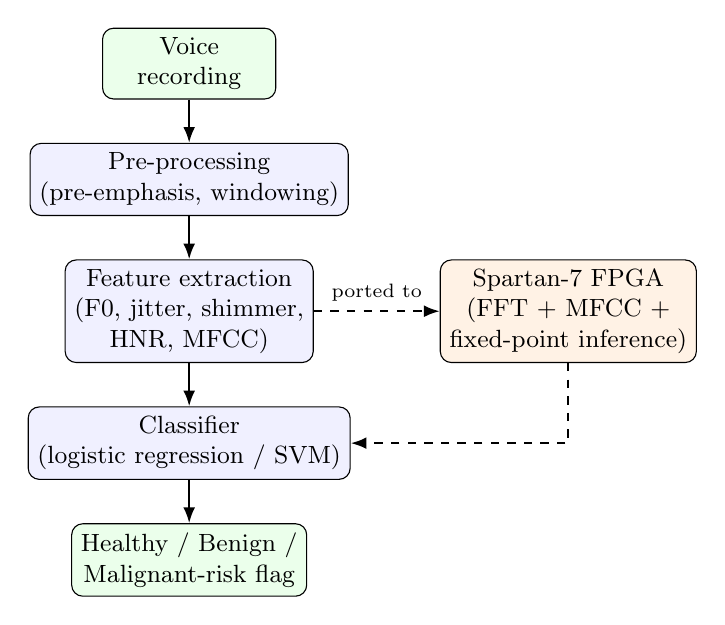
\begin{tikzpicture}[
    node distance=0.55cm and 0.9cm,
    block/.style={rectangle, draw, rounded corners, minimum width=2.5cm, minimum height=0.9cm, align=center, font=\small, fill=blue!6},
    io/.style={rectangle, draw, rounded corners, minimum width=2.2cm, minimum height=0.8cm, align=center, font=\small, fill=green!8},
    arr/.style={-{Latex[length=2mm]}, thick}
]
\node[io] (mic) {Voice \\ recording};
\node[block, below=of mic] (pre) {Pre-processing \\ (pre-emphasis, windowing)};
\node[block, below=of pre] (feat) {Feature extraction \\ (F0, jitter, shimmer, \\ HNR, MFCC)};
\node[block, below=of feat] (clf) {Classifier \\ (logistic regression / SVM)};
\node[io, below=of clf] (out) {Healthy / Benign / \\ Malignant-risk flag};

\draw[arr] (mic) -- (pre);
\draw[arr] (pre) -- (feat);
\draw[arr] (feat) -- (clf);
\draw[arr] (clf) -- (out);

\node[block, right=1.6cm of feat, fill=orange!10, minimum width=2.6cm] (fpga) {Spartan-7 FPGA \\ (FFT + MFCC + \\ fixed-point inference)};
\draw[arr, dashed] (feat.east) -- (fpga.west) node[midway, above, font=\scriptsize] {ported to};
\draw[arr, dashed] (fpga.south) |- (clf.east) node[near start, below, font=\scriptsize]{};
\end{tikzpicture}
\caption{Proposed system pipeline: a software baseline (solid path) extracts classical acoustic features and classifies healthy vs.\ benign vs.\ malignant-risk voices; the feature-extraction and inference stages are then targeted for real-time acceleration on a Xilinx Spartan-7 FPGA (dashed path).}
\label{fig:pipeline}
\end{figure}

\subsection{Timeline}
Table~\ref{tab:timeline} maps the stages above onto the deadlines specified in the project flier.

\begin{table}[h]
\centering
\caption{Project timeline mapped to grading milestones}
\label{tab:timeline}
\begin{tabular}{@{}p{2.1cm}p{2.0cm}p{3.4cm}@{}}
\toprule
\textbf{Deadline} & \textbf{Milestone} & \textbf{Deliverable} \\
\midrule
27.09.2026 & Preliminary report & Problem statement, literature review (this report) \\
25.10.2026 & Mid-term report & Data pipeline, classical feature extraction, baseline classifier replication, preliminary results, code \\
13.11.2026 & Final report & Improved classifier, class-imbalance handling, FPGA feature-extraction prototype, full results, code \\
TBD & Presentation/viva & Live demonstration and defence \\
\bottomrule
\end{tabular}
\end{table}

\section{Conclusion}
\label{sec:conclusion}
This report has motivated and formulated the problem of non-invasive laryngeal cancer screening from sustained-vowel voice recordings, framed as a signal-processing task centred on classical acoustic features (jitter, shimmer, HNR, MFCCs) rather than opaque raw-waveform deep learning. Our review of the literature shows that while voice-pathology detection on the Saarbr\"ucken Voice Database is well studied, the specific malignant-versus-benign distinction relevant to cancer screening is addressed by comparatively little work, and real-time or embedded realisation is, to our knowledge, unaddressed. Our project targets both gaps: isolating the malignant/pre-malignant SVD subset as an explicit classification target, and planning a Xilinx Spartan-7 FPGA implementation of the feature-extraction and inference pipeline. The next stage of the project will focus on implementing and validating the software feature-extraction and classification pipeline ahead of the mid-term report.

\section*{AI Usage Disclosure}
In accordance with the course AI usage policy, an AI assistant (Claude, Anthropic) was used to (i) assist in searching for and summarising related literature during the drafting of Section~\ref{sec:litreview}, and (ii) assist in structuring and formatting this LaTeX report. All technical claims drawn from external sources are cited to their original publications, and all AI-assisted content has been reviewed by the team members, who are prepared to explain and defend it during the project presentation and viva.

\begin{thebibliography}{00}

\bibitem{harar2017} P. Harar, J. B. Alonso-Hern\'andez, J. Mekyska, Z. Gal\'a\v{z}, R. Burget, and Z. Sm\'ekal, ``Voice pathology detection using deep learning: a preliminary study,'' in \emph{Proc. 5th IEEE Int. Work Conf. Bio-Inspired Intelligence (IWOBI)}, Funchal, Portugal, 2017, pp. 45--48, doi: 10.1109/IWOBI.2017.7985525.

\bibitem{mohammed2020} M. A. Mohammed, K. H. Abdulkareem, S. A. Mostafa, M. K. A. Ghani, M. S. Maashi, B. Garc\'ia-Zapirain, I. Oleagordia Ruiz, H. Alhakami, and F. T. Al-Dhief, ``Voice pathology detection and classification using convolutional neural network model,'' \emph{Applied Sciences}, 2020.

\bibitem{ksibi2023} A. Ksibi, N. A. Hakami, N. Alturki, M. M. Asiri, M. Zakariah, and M. Ayadi, ``Voice pathology detection using a two-level classifier based on combined CNN--RNN architecture,'' \emph{Sustainability}, vol. 15, no. 4, p. 3204, 2023.

\bibitem{lee2021} J.-Y. Lee, ``Experimental evaluation of deep learning methods for an intelligent pathological voice detection system using the Saarbr\"ucken voice database,'' \emph{Applied Sciences}, vol. 11, no. 15, p. 7149, 2021, doi: 10.3390/app11157149.

\bibitem{paterson2024} M. Paterson, J. Moor, and L. Cutillo, ``A classification benchmark for artificial intelligence detection of laryngeal cancer from patient voice,'' \emph{arXiv preprint arXiv:2412.16267}, 2024.

\bibitem{islam2022} R. Islam, E. Abdel-Raheem, and M. Tarique, ``Voice pathology detection using convolutional neural networks with electroglottographic (EGG) and speech signals,'' \emph{Computer Methods and Programs in Biomedicine Update}, vol. 2, p. 100074, 2022.

\end{thebibliography}

\end{document}
